\chapter{Eksplorasi Streaming Pesan Twitter, Sistem Hadoop, Hive dan Sqoop}

\section{Eksperimen}
Pada bagian ini, dilakukan uji coba beberapa kasus sederhana yang masih berhubungan dengan proses analisis teks pada sosial media Twitter. Eksperimen yang dilakukan seperti membuat program Java untuk melakukan \textit{streaming} data melalui Streaming API Twitter dan menyimpan hasilnya ke dalam file teks. Selain itu dilakukan juga eksperimen untuk melakukan pra pengolahan teks sederhana pada data tweet di lingkungan Hadoop.

\subsection{Streaming Tweet}
Dalam penelitian ini dibutuhkan tweet-tweet yang berhubungan dengan kegiatan pariwisata. Oleh karena itu dibuatlah sebuah program sederhana berbasis Java untuk melakukan streaming tweet. Kode sumber untuk eksperimen ini dapat dilihat pada Lampiran \ref{app:B}. Pada proses streaming tweet penulis menggunakan kata kunci libur, liburan, travel, travelling, wisata, tour, pariwisata, dan destinasi. Data tweet yang diambil juga dibatasi berdasarkan bahasa yang digunakan, hanya yang dalam bahasa Indonesia saja yang diambil. Berikut adalah salah satu contoh hasil tweet yang dihasilkan.

\begin{lstlisting}[language=Java,basicstyle=\tiny,caption=Hasil Streaming]
{
  "created_at": "Mon Sep 28 00:48:47 +0000 2015",
  "id": 6.4829827034363e+17,
  "id_str": "648298270343626752",
  "text": "Ujudkan ikon Pariwisata berwawasan lingkungan. Bali sdh banyak bermasalah dg air, fungsi lahan, dan sampah. http:\/\/t.co\/mj8l3D4xvy #AjegBali",
  "source": "<a href=\"http:\/\/twitter.com\/download\/iphone\" rel=\"nofollow\">Twitter for iPhone<\/a>",
  "truncated": false,
  "in_reply_to_status_id": null,
  "in_reply_to_status_id_str": null,
  "in_reply_to_user_id": null,
  "in_reply_to_user_id_str": null,
  "in_reply_to_screen_name": null,
  "user": {
    "id": 1690141351,
    "id_str": "1690141351",
    "name": "Bali Tolak Reklamasi",
    "screen_name": "ForBALI13",
    "location": "Bali",
    "url": "http:\/\/forbali.org",
    "description": "Official account Forum Rakyat Bali #TolakReklamasiTelukBenoa | Petisi: http:\/\/chn.ge\/1kyV5Bu | Ganti Profpic: http:\/\/twibbon.com\/support\/forbali-2",
    "protected": false,
    "verified": false,
    "followers_count": 43317,
    "friends_count": 178,
    "listed_count": 21,
    "favourites_count": 388,
    "statuses_count": 11135,
    "created_at": "Thu Aug 22 05:27:11 +0000 2013",
    "utc_offset": 21600,
    "time_zone": "Urumqi",
    "geo_enabled": false,
    "lang": "en",
    "contributors_enabled": false,
    "is_translator": false,
    "profile_background_color": "C0DEED",
    "profile_background_image_url": "http:\/\/pbs.twimg.com\/profile_background_images\/378800000077490261\/b733ff1364e61ccf11b48d972a419799.jpeg",
    "profile_background_image_url_https": "https:\/\/pbs.twimg.com\/profile_background_images\/378800000077490261\/b733ff1364e61ccf11b48d972a419799.jpeg",
    "profile_background_tile": true,
    "profile_link_color": "0084B4",
    "profile_sidebar_border_color": "FFFFFF",
    "profile_sidebar_fill_color": "DDEEF6",
    "profile_text_color": "333333",
    "profile_use_background_image": true,
    "profile_image_url": "http:\/\/pbs.twimg.com\/profile_images\/494053969430200320\/X2xjdPf-_normal.png",
    "profile_image_url_https": "https:\/\/pbs.twimg.com\/profile_images\/494053969430200320\/X2xjdPf-_normal.png",
    "profile_banner_url": "https:\/\/pbs.twimg.com\/profile_banners\/1690141351\/1402672316",
    "default_profile": false,
    "default_profile_image": false,
    "following": null,
    "follow_request_sent": null,
    "notifications": null
  },
  "geo": null,
  "coordinates": null,
  "place": null,
  "contributors": null,
  "retweet_count": 0,
  "favorite_count": 0,
  "entities": {
    "hashtags": [
      {
        "text": "AjegBali",
        "indices": [
          131,
          140
        ]
      }
    ],
    "trends": [
      
    ],
    "urls": [
      {
        "url": "http:\/\/t.co\/mj8l3D4xvy",
        "expanded_url": "http:\/\/bit.ly\/1PIgk0x",
        "display_url": "bit.ly\/1PIgk0x",
        "indices": [
          108,
          130
        ]
      }
    ],
    "user_mentions": [
      
    ],
    "symbols": [
      
    ]
  },
  "favorited": false,
  "retweeted": false,
  "possibly_sensitive": false,
  "filter_level": "low",
  "lang": "in",
  "timestamp_ms": "1443401327106"
}
\end{lstlisting}

Proses yang dilakukan pada eksperimen ini adalah
\begin{enumerate}
	\item Mendaftar di https://dev.twitter.com/ untuk mendapatkan \textit{consumer key,  consumer secret, access token,} dan \textit{access token secret} yang akan digunakan untuk mendapatkan data dari Twitter Streaming API.
	\item Membuat program Java dengan bantuan library org.scribe versi 1.3.7 yang berfungsi untuk melakukan autentikasi OAuth ke server Twitter.
	\item Mendapatkan tweet yang dikirim Twitter Streaming Server dan menyimpannya ke dalam file text.
\end{enumerate}
 
Dari hasil eksperimen ini ada beberapa hal yang perlu dievaluasi dan dikembangkan, yaitu:

\begin{itemize}
	\item Penulisan hasil streaming tweet langsung ke HDFS.
\end{itemize}


\subsection{\textit{Text Preprocessing} Tweet Sederhana di Lingkungan Hadoop}
Untuk melakukan pengolahan pada tweet perlu diawali dengan \textit{text preprocessing} terlebih dahulu. Oleh karena itu perlu dilakukan eksperimen untuk melakukan text preprocessing sederhana pada data tweet di lingkungan sistem terdistribusi Hadoop. Kode sumber untuk eksperimen ini dapat dilihat pada Lampiran \ref{app:C}. Berikut adalah proses yang dilakukan pada eksperimen ini.

\begin{enumerate}
	\item Mengubah text ke dalam huruf kecil.
	\item Membuang stopwords pada tweet. Daftar stopwords yang digunakan dapat dilihat di Lampiran \ref{app:A}.
	\item Membuang tag ke pengguna lain (diawali dengan @) dan hashtag topik tertentu (diawali dengan \#).
	\item Membuang URL yang terdapat pada tweet.
	\item Menghilangkan karakter-karakter lainnya selain alfabet dari A sampai Z atau angka 0 sampai 9.
	\item Membuan spasi di awal dan akhir tweet serta menghilangkan multiple spasi.
\end{enumerate}
 
Untuk mendukung proses tersebut di atas dibutuhkan \textit{library} pendukung lainnya yaitu org.apache.hadoop versi 2.7.1. Berikut adalah beberapa contoh masukan dan keluaran dari program sederhana ini.\\
 
     
\textbf{Masukan:}
\begin{enumerate}
	\item RT @CJRisCJR: Mau liburan ke Jepang bareng kita?Yuk ikut \#BoneetoTemuinKerenmu dari @BoneetoID ! Info, klik  http://t.co/THYLKLnSbX http://?
	\item @Hai @dimasarasta  Lets Joint With Us Wisata Seluler ke Jantungnya XL http://t.co/VPO4QyOBOt
	\item WISATA PULAU TIDUNG- Pemerintah Pusat Tetapkan Pantai Rupat jadi Tujuan Wisata Nasional - Metroterkini  http://t.co/LCUZJQveuX
	\item Paket Tour Karimunjawa 3hari 2malam | Mulai 805k/pax, min 8 pax | MoreInfo: 0271-733176, WA 089602910275, BB 5A4CC077 http://t.co/bc7os4f35J
	\item RT @detikcom: Ini Dampak Kabut Asap Terhadap Tour de Singkarak 2015 http://t.co/lNbnyPB485  via @detiktravel
\end{enumerate} 
     
\textbf{Keluaran:}
\begin{enumerate}
	\item liburan jepang bareng yuk info klik 
	\item lets joint with us wisata seluler jantungnya xl
	\item wisata pulau tidung pemerintah pusat tetapkan pantai rupat tujuan wisata nasional metroterkini
	\item paket tour karimunjawa 3hari 2malam 805kpax min 8 pax moreinfo 0271733176 wa 089602910275 bb 5a4cc077
	\item dampak kabut asap tour de singkarak 2015 via
\end{enumerate}

  
Dari hasil eksperimen ini ada beberapa hal yang perlu dievaluasi dan dikembangkan, yaitu:
\begin{itemize}
	\item Menghilangkan angka pada tweet, karena tidak dapat dimanfaatkan dalam proses text mining untuk mendapatkan sentimen tweetnya.
	\item Menambahkan daftar kata stopwords.
	\item Mengatasi penggunaan bahasa slang dan singkatan kata.
\end{itemize}

\subsection{Eksperimen dengan Hive}
\label{sec:eksperimen-hive}
Pada eksperimen kali ini akan dibuat beberapa kode program sederhana untuk melakukan percobaan membuat tabel, mengimpor data ke dalam tabel, dan membaca isi dari tabel. Eksperimen ini menggunakan driver JDBC (org.apache.hive.jdbc.HiveDriver) untuk melakukan koneksi dari program java ke Hive. 

Berikut adalah salah satu kueri yang dijalankan pada Hive untuk membuat sebuah tabel baru bernama tweets. Tabel tweets memiliki atribut source\_id, text, geo, dan place yang bertipe String dan timestamp\_ms dengan tipe data Big Integer. Setiap \textit{record} pada tabel tweets dipisahkan dengan baris baru dan nilai dari setiap kolom-kolomnya akan dipisahkan dengan tab.

\begin{lstlisting}[language=sql,basicstyle=\small,caption=Kueri Hive untuk Membuat Tabel tweets]
CREATE TABLE tweets (
    source_id STRING
    text STRING
    geo STRING
    place STRING
    timestamp_ms BIGINT
) 
ROW FORMAT DELIMITED 
FIELDS TERMINATED BY '\t'
\end{lstlisting}

Kueri di atas akan dijalankan bersama beberapa kueri lainnya di dalam sebuah program java (PrepareHiveTable.java). Sumber kode lengkapnya dapat dilihat pada Lampiran \ref{app:D}. Ketika program dijalankan maka akan mengeluarkan output seperti pada Gambar \ref{fig:output-preparetable-hive} yang artinya tabel baru berhasil dibuat di dalam Hive. 

\begin{figure}
	\centering
	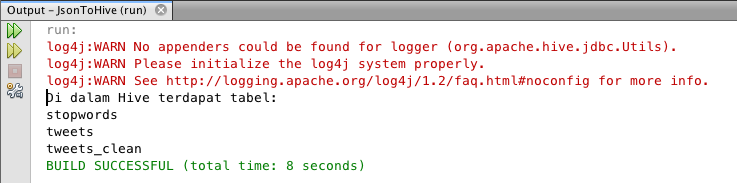
\includegraphics[scale=0.5]{Gambar/output-preparetable-hive.png}
	\caption[Keluaran dari program PrepareHiveTable.java]{Keluaran dari program PrepareHiveTable.java}
	\label{fig:output-preparetable-hive}
\end{figure}

Untuk memastikan tabel yang dibuat sudah benar sesuai dengan kueri yang dibuat di dalam program maka dilakukan pengecekan langsung ke dalam \textit{Command Line Interface} (CLI) dari Hive. Pertama-tama dilakukan pengecekan tabel-tabel yang dibuat menggunakan kueri SHOW TABLES. Keluaran dari kueri ini seperti pada Gambar \ref{fig:show-tables-hive} yang artinya terdapat tiga buah tabel di dalam Hive bernama stopwords, tweets, dan tweets\_clean.

\begin{figure}
	\centering
	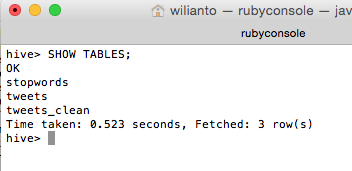
\includegraphics[scale=1]{Gambar/show-tables-hive.png}
	\caption[Keluaran Tabel-tabel Hive]{Keluaran Tabel-tabel Hive}
	\label{fig:show-tables-hive}
\end{figure}

Selanjunya dilakukan pengecekan kolom dan tipe data pada tabel-tabel yang sudah berhasil dibuat. Kueri yang digunakan untuk melakukan pengecekan ini adalah DESC nama\_tabel. Keluaran dari kueri ini dapat dilihat pada Gambar \ref{fig:desc-tables-hive}. Jika dibandingkan keluaran yang dihasilkan memiliki nama kolom dan tipe data yang sesuai dengan kueri pada program PrepareHiveTable.java. Maka dapat disimpulkan program PrepareHiveTable.java berjalan dengan baik dan berhasil membuat tabel Hive.

\begin{figure}
	\centering
	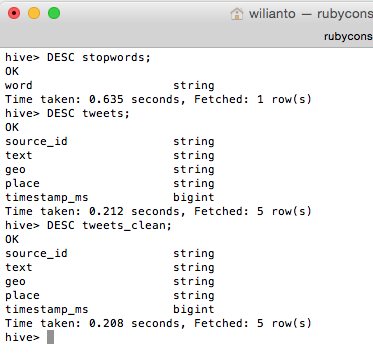
\includegraphics[scale=1]{Gambar/desc-tables-hive.png}
	\caption[Keluaran Kolom-kolom pada Tabel Hive]{Keluaran Kolom-kolom pada Tabel Hive}
	\label{fig:desc-tables-hive}
\end{figure}

Setelah tabel berhasil dibuat ekperimen berikutnya adalah memasukan data ke dalam Hive. Dalam ekperimen ini akan ada dua buah tabel yang diisi, yaitu tabel tweets dan stopwords. Skenario yang digunakan pada ekperimen kali ini adalah memasukan data-data dengan format tertentu dari file tweets.txt dan stopwords.txt menggunakan kueri LOAD dari Hive. Sumber kode penuh dan file-file yang diperlukan untuk proses impor data ke dalam Hive ini dapat dilihat pada Lampiran \ref{app:D}. 

\begin{lstlisting}[language=sql,basicstyle=\tiny,caption=Kueri Hive untuk Import Data dari File]
LOAD DATA LOCAL INPATH '/Users/wilianto/Documents/MyDocuments/software/mac/trial-data/stopwords.txt'
OVERWRITE INTO TABLE stopwords
\end{lstlisting}

Keluaran dari program ImportTweets.java dan ImportStopWords.java digambarkan pada Gambar \ref{fig:hasil-impor-tweets} dan \ref{fig:hasil-impor-stopwords}. Setelah program berhasil dijalankan maka dilakukan pengecekan langsung ke Hive CLI untuk melihat data-data yang berhasil dimasukan. Keluaran dari kueri yang dilakukan untuk menampilkan seluruh isi data dari kedua tabel dapat dilihat pada Gambar \ref{fig:cek-hasil-impor-hive}.

\begin{figure}
	\centering
	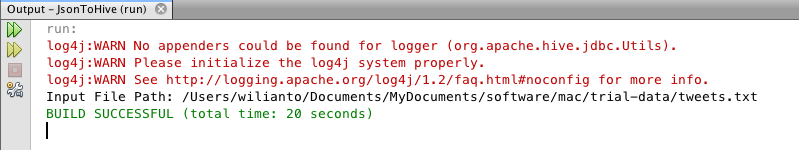
\includegraphics[scale=0.5]{Gambar/hasil-impor-tweets.png}
	\caption[Keluaran Impor Data Tweets]{Keluaran Impor Data Tweets}
	\label{fig:hasil-impor-tweets}
\end{figure}

\begin{figure}
	\centering
	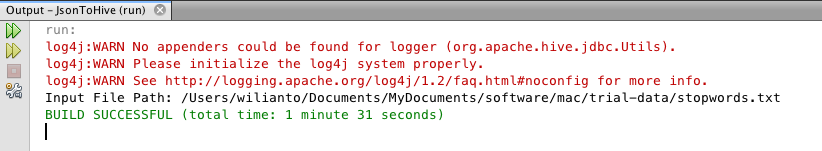
\includegraphics[scale=0.5]{Gambar/hasil-impor-stopwords.png}
	\caption[Keluaran Impor Data Stopwords]{Keluaran Impor Data Stopwords}
	\label{fig:hasil-impor-stopwords}
\end{figure}

\begin{figure}
	\centering
	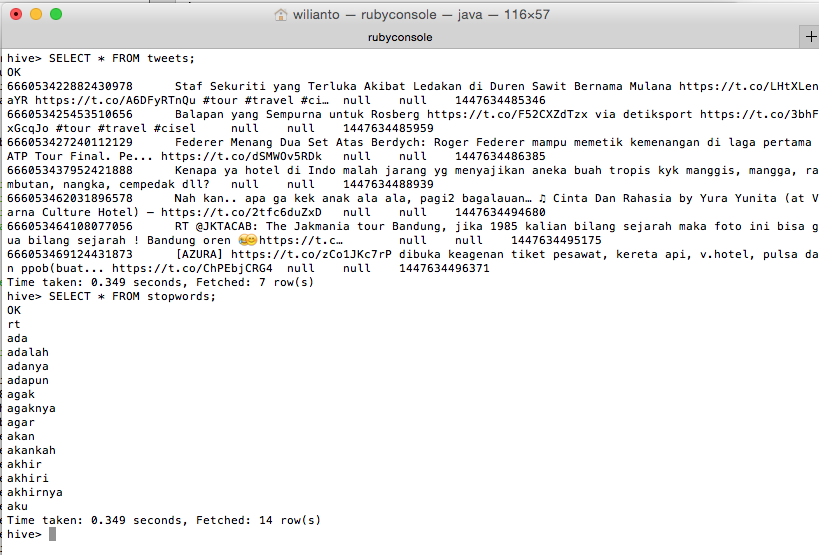
\includegraphics[scale=0.5]{Gambar/cek-hasil-impor-hive.png}
	\caption[Keluaran dari Kueri Select untuk Tabel tweets dan stopwords pada Hive]{Keluaran dari Kueri Select untuk Tabel tweets dan stopwords pada Hive}
	\label{fig:cek-hasil-impor-hive}
\end{figure}


\subsection{Eksperimen dengan Sqoop}
\label{sec:eksperimen-sqoop}
Ekperimen Sqoop dilakukan untuk mencoba proses impor dan ekpor data ke dalam HDFS khususnya menggunakan Hive. Berikut adalah perintah-perintah yang digunakan untuk melakukan proses impor dan ekspor. Parameter --connect digunakan untuk melakukan koneksi ke basis data lain menggunakan konektor Sqoop dan JDBC. --username, --password adalah data-data yang diperlukan untuk melakukan akses ke dalam basisdata. --table adalah tabel asal yang akan diimpor datanya. --hive-import digunakan untuk menandakan bahwa data yang diimpor akan disimpan dalam bentuk tabel hive, apabila parameter ini tidak digunakan maka data akan disimpan sebagai file teks biasa di HDFS. --bindir adalah lokasi direktori tempat file java otomatis dibuat oleh Sqoop. --fields-terminated-by dan --lines-terminated-by digunakan untuk pemisah antar nilai \textit{field} dan pemisah antar \textit{record}. Hasil dari proses impor berhasil dibuktikan pada Gambar \ref{fig:cek-hasil-impor-sqoop}, terdapat 28.526 data yang berhasil diimpor.

\begin{lstlisting}[basicstyle=\tiny,caption=Perintah Sqoop untuk Melakukan Impor]
bin/sqoop import \
--connect jdbc:mysql://127.0.0.1:3306/skripsi_data \
--username root \
--password admin123 \
--table tb_katadasar \
--hive-import \
--bindir /Users/wilianto/Documents/MyDocuments/software/mac/sqoop-1.4.6.bin__hadoop-2.0.4-alpha \
--fields-terminated-by ',' \
--lines-terminated-by '\n'
\end{lstlisting}

\begin{figure}
	\centering
	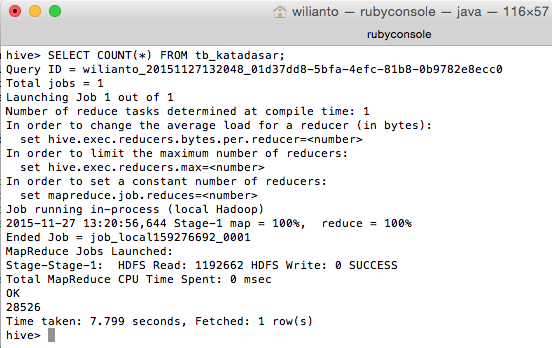
\includegraphics[scale=0.5]{Gambar/cek-hasil-impor-sqoop.png}
	\caption[Mencari Jumlah Data yang Berhasil Diimpor oleh Sqoop]{Mencari Jumlah Data yang Berhasil Diimpor oleh Sqoop}
	\label{fig:cek-hasil-impor-sqoop}
\end{figure}

Parameter yang digunakan untuk proses ekspor hampir sama dengan yang digunakan untuk proses impor. Yang menjadi pembeda hanya pada parameter --hive-import yang tidak perlu lagi dituliskan, parameter --table di sini berfungsi untuk menunjuk tabel di basis data relasional yang akan dituju dan ada penambahan parameter --export-dir yang berguna untuk menunjuk direktori data yang akan diekspor di dalam HDFS. Hasil dari proses ekspor berhasil dibuktikan pada Gambar \ref{fig:cek-hasil-ekspor-sqoop}, terdapat 28.526 data yang berhasil diekspor.

\begin{lstlisting}[basicstyle=\tiny,caption=Perintah Sqoop untuk Melakukan Ekspor]
bin/sqoop export \
--connect jdbc:mysql://127.0.0.1:3306/skripsi_data \
--username root \
--password admin123 \
--table tb_katadasar_from_hive \
--export-dir /user/hive/warehouse/tb_katadasar \
--bindir /Users/wilianto/Documents/MyDocuments/software/mac/sqoop-1.4.6.bin__hadoop-2.0.4-alpha \
--fields-terminated-by ',' \
--lines-terminated-by '\n'
\end{lstlisting}

\begin{figure}
	\centering
	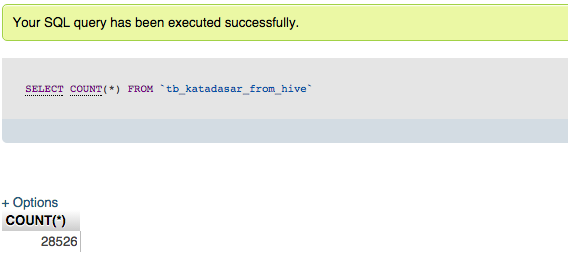
\includegraphics[scale=0.5]{Gambar/cek-hasil-ekspor-sqoop.png}
	\caption[Mencari Jumlah Data yang Berhasil Diekspor oleh Sqoop]{Mencari Jumlah Data yang Berhasil Diekspor oleh Sqoop}
	\label{fig:cek-hasil-ekspor-sqoop}
\end{figure}
